\documentclass[12pt,a4paper]{report}

% ------------ PACKAGE SETTINGS -----------------
\usepackage{graphicx}
\usepackage{float}
\usepackage{setspace}
\usepackage{geometry}
\usepackage{tocloft}
\usepackage{titlesec}
\usepackage{lipsum}
\usepackage{hyperref}

% Page margins
\geometry{
    left=1.25in,
    right=1in,
    top=1in,
    bottom=1in
}

% Line spacing
\onehalfspacing

% ------------ BEGIN DOCUMENT -----------------
\begin{document}

% -----------------------------------------------
% ROMAN NUMBERING FOR PRELIMINARY PAGES
% -----------------------------------------------
\pagenumbering{roman}
\setcounter{page}{1}

% ------------ TITLE PAGE (NO PAGE NUMBER) ------
\begin{titlepage}
    \thispagestyle{empty}
    \centering
    {\Large \textbf{PROJECT DOCUMENTATION}}\\[1cm]

    {\Large \textbf{Traffic Monitoring System: Real-Time Detection and Classification of Nepali Vehicles}}\\
    {\large Submitted in partial fulfillment of the requirement of
Computer Project-II (BCE5017)
}\\[0.4cm]
\begin{figure}[H]
    \centering
    
\includegraphics[width=0.4\textwidth]{Purbanchal University Logo.jpg}
\end{figure}
{\large Purbanchal University}\\[0.5cm]
{\large Birtanagar, Nepal}\\[0.5cm]

    
    {\large \textbf{Submitted by:}}\\[0.2cm]
    {\large {Sangam Panday (Roll No.)}}\\
    {\large {Sandesh Neupane (Roll No.)}}\\
    {\large {Spriha Bhattarai (Roll No.)}}\\[1.5cm]

    {\large \textbf{Department of Computer Engineering}}\\
    {\large Kantipur City College}\\


    \vfill
    {\large \textbf{May, 2026}}
\end{titlepage}

%--------------TItle page ii----------------------
\begin{titlepage}
    \thispagestyle{empty}
    \centering
    {\Large \textbf{PROJECT DOCUMENTATION}}\\[1cm]

    {\Large \textbf{Traffic Monitoring System: Real-Time Detection and Classification of Nepali Vehicles}}\\
    {\large Submitted in partial fulfillment of the requirement of
Computer Project-II (BCE5017)
}\\[0.4cm]
{\large \textbf{Submitted to:}}\\[0.5cm]
{\large Purbanchal University}\\[0.5cm]
{\large Birtanagar, Nepal}\\[0.5cm]

    
    {\large \textbf{Submitted by:}}\\[0.2cm]
    {\large {Sangam Panday (Roll No.)}}\\
    {\large {Sandesh Neupane (Roll No.)}}\\
    {\large {Spriha Bhattarai (Roll No.)}}\\[1.5cm]

    {\large \textbf{Project Supervisor:}}\\[0.5cm]
{\large Sagar Dhakal}\\[0.5cm]

    {\large \textbf{Department of Computer Engineering}}\\
    {\large Kantipur City College}\\


    \vfill
    {\large \textbf{May, 2026}}
\end{titlepage}

% ------------ DECLARATION PAGE -----------------
\chapter*{Declaration}
\addcontentsline{toc}{chapter}{Declaration}

We hereby declare that this project report entitled "\textbf{Traffic Monitoring System: Real-Time Detection and Classification of Nepali Vehicles}" submitted to the Department of Computer Engineering is our original work and has not been submitted elsewhere for the award of any degree..

\vspace{1cm}
\noindent\textbf{Sangam Panday}\\
\textbf{Sandesh Neupane}\\
\textbf{Spriha Bhattarai}

\newpage

% ------------ ACKNOWLEDGMENT -----------------
\chapter*{Acknowledgment}
\addcontentsline{toc}{chapter}{Acknowledgment}

We would like to express our sincere gratitude to Er. Sagar Dhakal for his invaluable guidance and support throughout this project. We also thank the Department of Computer Engineering at Kantipur City College for providing the necessary resources and facilities. We are grateful to all those who contributed to the successful completion of this Nepali-specific vehicle classification system, particularly those involved in data collection from Nepali traffic scenarios and testing the system in diverse Nepali urban environments.

\vspace{1cm}
\begin{flushright}
\textbf{Sangam Panday}\\
\textbf{Sandesh Neupane}\\
\textbf{Spriha Bhattarai}
\end{flushright}

\newpage

% ------------ ABSTRACT PAGE -----------------
\chapter*{Abstract}
\addcontentsline{toc}{chapter}{Abstract}

This project presents an automated vehicle classification system specifically designed and trained for Nepali traffic conditions. It detects and categorizes vehicles from video and image inputs using computer vision and custom machine learning models. The system identifies and classifies Nepali vehicles into predefined categories including cars, motorcycles, buses, trucks, and other common vehicle types found in Nepali urban and highway traffic. Unlike generic vehicle detection systems trained on international datasets, this system is specifically optimized for Nepali traffic scenarios \cite{tak2021development}. The project is built using Python, Flask, and a custom-trained vehicle classifier model fine-tuned on Nepali traffic datasets. The system processes video frames, applies YOLOv8 vehicle detection algorithms, classifies detected vehicles using the custom Nepali classifier, tracks vehicles across frames using DeepSORT, detects vehicle colors, and generates detailed reports in CSV format. Additionally, the system includes a web-based interface for easy interaction and result visualization, enabling traffic authorities and researchers to analyze Nepali traffic patterns effectively. The project demonstrates the practical application of artificial intelligence and computer vision in solving traffic monitoring challenges specific to Nepal, offering a scalable, localized solution for traffic analysis and vehicle tracking applications in Nepali cities.

\newpage
%---------Supervisor's Approval---------------------
\chapter*{Supervisor Approval}
\addcontentsline{toc}{chapter}{Supervisor's Approval}

This is to certify that this semesters  the project entitled “Traffic Monitoring System: Real-Time Detection and Classification of Nepali Vehicles” undertaken and demonstrated by Sangam Panday, Spriha Bhattarai and Sandesh Neupane, has been successfully completed under my supervision as a partial fulfillment of the requirements of the degree of Computer Engineering 5th semester under Purbanchal University. I, henceforth, approve this project to be awarded the certificate by the concerned authority. 

During supervision, I found students hardworking, skilled and ready to undertake any professional work related to this field in the future.


\vspace{4cm}
\noindent
\begin{minipage}{0.5\textwidth}
  \rule{5cm}{0.4pt}\\ [0.2cm]
  \textbf{Er Sagar Dhakal}\\
  \textbf{Project Supervisor}\\
  \textbf{Kantipur City College}
\end{minipage}


\newpage

%-------------Certification from department--------------------
\chapter*{Certification from department}
\addcontentsline{toc}{chapter}{Certificate from Department}

Following the Supervisor's Approval and Examiners' Acceptance, the project entitled “Traffic Monitoring System: Real-Time Detection and Classification of Nepali Vehicles" submitted by Sangam Panday, Spriha Bhattarai and Sandesh Neupane, as a partial fulfillment of the requirements for the degree of Computer Engineering 5th semester under Purbanchal University, has been officially awarded by this certificate.

 I wish the students all the best for their future endeavors.



\vspace{4cm}
\noindent
\begin{minipage}{0.8\textwidth}
  \rule{5cm}{0.4pt}\\ [0.2cm]
  \textbf{Er Subash Rajkarnikar}\\
  \textbf{Head of Department}\\
  \textbf{Department of Computer Engineering}\\
  \textbf{Kantipur City College}
\end{minipage}


\newpage

% ------------ TABLE OF CONTENTS -----------------
\tableofcontents
\newpage

% ------------ LIST OF FIGURES & TABLES ---------
\listoffigures
\newpage

\listoftables
\newpage

% -----------------------------------------------
% SWITCH TO ARABIC NUMBERING FOR CHAPTERS
% -----------------------------------------------
\pagenumbering{arabic}
\setcounter{page}{1}

% ------------ CHAPTER 1 -----------------
\chapter{Introduction}

\section{Overview}
The Nepali vehicle classification system addresses the specific challenges of Nepali traffic monitoring, where diverse vehicle types including hiace, motorcycles, and various bus configurations are prevalent. Unlike generic vehicle detection systems trained on international datasets \cite{sivaraman2016detecting}, this system is specifically optimized for Nepali urban and highway traffic scenarios, accounting for local vehicle types, traffic patterns, and environmental conditions typical to Nepal.

The Traffic Monitoring System is an intelligent web-based platform designed to automatically detect and classify vehicles from video and image inputs captured in Nepali traffic environments. With increasing urbanization and traffic congestion in cities like Kathmandu, Pokhara, and other Nepali urban centers, the need for efficient traffic monitoring has become critical. Traditional manual traffic monitoring is time-consuming, prone to human error, and cannot handle the volume of data generated by modern surveillance systems in Nepal.

This project includes an efficient deep learning model that can automatically recognize and categorize vehicles based on their visual features. It uses advanced image processing techniques and convolutional neural networks (CNN) \cite{krizhevsky2012imagenet} where the system learns patterns and categorizes vehicles by their unique characteristics. The system is built using the YOLOv8 (You Only Look Once version 8) model \cite{redmon2016yolo, ultralytics2023yolov8} for detection combined with a custom-trained Nepali vehicle classifier that has been specifically trained on Nepali traffic datasets. Through this training process on local data, the model learns to distinguish between different Nepali vehicle categories based on features such as shape, structure, size, and visual patterns characteristic of vehicles found in Nepal. Additionally, the system incorporates DeepSORT tracking \cite{bewley2016deepsort} to maintain consistent vehicle identities across video frames and automated color detection to provide comprehensive traffic analytics. The system is trained specifically on Nepali vehicle datasets, enabling it to recognize vehicle types and traffic patterns unique to Nepal, including auto-rickshaws, local bus variants, and motorcycles commonly used in Nepali transportation.

\section{Problem Statement}

In Nepal, identifying and classifying the diverse range of vehicles—including cars, motorcycles, auto-rickshaws, buses, and trucks—from traffic surveillance footage is particularly challenging due to varied lighting conditions, urban congestion, and the diversity of vehicle types common to Nepali streets. Manual monitoring is highly time-consuming, prone to human error, and inadequate for analyzing large volumes of traffic surveillance data from Nepali cities and highways \cite{tak2021development}. There is a critical need for a Nepali vehicle-specific automated system that accurately recognizes and categorizes the unique vehicle types found in Nepali traffic. Additionally, extracting meaningful insights from vehicle classification data requires advanced querying and analytical capabilities that are difficult to achieve manually.

Generic vehicle detection systems trained on international datasets often fail to perform optimally on Nepali vehicles due to differences in vehicle designs, traffic patterns, and environmental conditions. This project addresses this critical gap by developing a system specifically trained on Nepali traffic data.

\section{Objectives}

\begin{itemize}
    \item The primary objective of this project is to design and develop an automated vehicle detection and classification system specifically trained and optimized for Nepali traffic conditions and vehicle types.
    
    \item The system aims to utilize custom-trained deep learning models specifically fine-tuned for Nepali vehicles to achieve high classification accuracy on local traffic data.
    
    \item To provide a user-friendly web interface that allows easy upload and processing of Nepali traffic video and image data.
    
    \item To generate detailed reports and analytics in CSV format with vehicle tracking, color detection, and trajectory information for further analysis by traffic authorities.
    
    \item To implement intelligent query mechanisms for analyzing classified Nepali vehicle data using advanced language models, enabling traffic pattern analysis and insights extraction.
\end{itemize}

\section{Features}

\begin{itemize}
    \item Automated Detection and Classification of Nepali Vehicle Types
    \item Multi-Object Tracking with DeepSORT for Consistent Vehicle ID Tracking
    \item Web-Based Dashboard for Result Visualization
    \item Advanced Query System for Analyzing Nepali Traffic Data
\end{itemize}

\section{Significance}

This project demonstrates the practical application of artificial intelligence and computer vision in solving real-world traffic monitoring challenges specific to Nepali urban and highway environments \cite{lecun2015deep}. By developing a system trained on Nepali traffic datasets that can automatically recognize and categorize local vehicle types—including auto-rickshaws, motorcycles, and various bus configurations—the project highlights how custom deep learning models can be adapted for regional contexts. This localization approach enables Nepal to implement cost-effective, open-source traffic monitoring solutions tailored to local transportation needs rather than relying solely on generic international systems.

The significance of this Nepali-specific approach is that it provides a foundation for understanding how AI systems need to be customized for different regional contexts and traffic conditions. Generic vehicle detection models may not perform optimally on Nepali vehicles and traffic patterns, making a localized solution valuable for Kathmandu, Pokhara, and other Nepali cities implementing modern traffic management systems.

The project is significant as it provides foundational knowledge for how image-based recognition systems can be adapted to regional contexts, especially in handling variations such as different lighting conditions, angles, distances, backgrounds, and the specific vehicle types found in Nepal. It also helps in building knowledge of model training on local datasets, data handling specific to Nepali traffic, performance evaluation in regional contexts, and real-time inference—all essential concepts in developing localized AI applications. Furthermore, the integration of query mechanisms with classification data provides traffic authorities and researchers with the ability to extract meaningful insights from large-scale Nepali traffic data.

\section{Scope and Limitations}

\subsection*{Scope}
\begin{itemize}
    \item Develops a deep learning-based system specifically for Nepali vehicle classification from images and video frames.
    \item Focuses on identifying Nepali-specific vehicle types: cars, motorcycles, auto-rickshaws, buses, trucks, and other local transportation vehicles.
    \item Trained and tested on Nepali traffic datasets representing typical Nepali urban and highway conditions.
    \item Includes processes such as Nepali vehicle data collection, preprocessing, custom model training, and prediction.
    \item Provides a web-based interface for uploading and processing Nepali traffic video and image data.
    \item Generates comprehensive CSV reports with Nepali vehicle detections, classifications, and tracking data.
    \item Implements advanced features like vehicle color detection and trajectory tracking for comprehensive traffic analysis.
    \item Suitable for integration into Nepali traffic monitoring and surveillance systems.
    \item Provides a framework that can be extended to include more Nepali vehicle categories and regional variations.
\end{itemize}

\subsection*{Limitations}
\begin{itemize}
    \item The model's accuracy depends heavily on the quality and size of the Nepali training dataset.
    \item It may not perform well on images or videos with poor lighting, low resolution, or heavy background noise typical in some Nepali traffic scenarios.
    \item The system is limited to the Nepali vehicle categories it has been trained on and cannot recognize unseen vehicle types without retraining.
    \item Real-time processing speed depends on the hardware available (CPU/GPU).
    \item The system works best with clear vehicle instances and may struggle with highly occluded or partially visible vehicles in congested Nepali traffic situations.
    \item Query capabilities are dependent on the completeness and quality of the classification data.
    \item Performance optimization for monsoon seasons and adverse weather common in Nepal requires additional model training and tuning.
\end{itemize}

\section{Organization of the Document}
This document is organized as follows: Chapter 1 presents the Introduction with Nepali context, Chapter 2 covers the Literature Review including Nepal-specific considerations, Chapter 3 describes the Methodology with Nepali customizations, Chapter 4 details System Analysis, Chapter 5 outlines System Design, Chapter 6 covers System Development and Implementation with Nepali vehicle features, Chapter 7 presents Testing Results on Nepali vehicles, Chapter 8 provides Conclusion and Future Work including Nepali deployment plans, and finally References including Nepali traffic studies.

% ------------ CHAPTER 2 -----------------
\chapter{Literature Review}

\section{Theoretical Review}

Modern vehicle detection and classification systems are built on theoretical foundations from computer vision and deep learning. According to research in the field of object detection \cite{lecun2015deep}, convolutional neural networks (CNNs) provide robust mechanisms for feature extraction and image classification. The theoretical framework for YOLO (You Only Look Once) architecture \cite{redmon2016yolo} demonstrates that real-time object detection is achievable by reformulating detection as a single regression problem, where bounding boxes and class probabilities are predicted directly from full images in one evaluation.

The theoretical literature emphasizes that effective vehicle classification systems require: (1) robust feature extraction through deep neural networks, (2) appropriate training data with diverse vehicle instances, (3) optimization techniques for model convergence, and (4) evaluation metrics such as precision, recall, and mean average precision (mAP). These concepts form the backbone of modern traffic monitoring systems that rely on computer vision.

Additionally, transfer learning techniques have demonstrated that pre-trained models can effectively adapt to specific vehicle classification tasks with reduced training time and improved accuracy \cite{krizhevsky2012imagenet}. The theoretical foundation supports the use of pre-trained YOLOv8 models for vehicle detection and classification tasks in traffic monitoring applications. Moreover, the theory of domain adaptation suggests that models fine-tuned on region-specific data significantly outperform generic international models when deployed in localized contexts.


\section{Empirical Review}

Empirical studies in vehicle detection and classification have shown that deep learning models significantly outperform traditional computer vision methods. Research on YOLOv8 \cite{ultralytics2023yolov8} demonstrates that this architecture achieves high accuracy in real-time object detection scenarios with minimal false positives.

Studies on vehicle classification systems show that users and system administrators strongly prefer automated approaches over manual monitoring due to increased efficiency and reduced human error. Field deployments of AI-based traffic monitoring systems \cite{tak2021development} have demonstrated improvements in traffic analysis accuracy and reduced operational costs.

Empirical evidence also supports the effectiveness of multi-class classification systems for distinguishing between diverse vehicle types. The literature indicates that systems incorporating visual feedback through bounding boxes and classification labels significantly improve interpretability and user confidence in results.

Furthermore, research on data-driven decision making in traffic management shows that systems providing exportable data in formats like CSV enable better downstream analysis and integration with other traffic management tools \cite{mckinney2010data}. Studies on multi-object tracking demonstrate that DeepSORT \cite{bewley2016deepsort} significantly improves vehicle trajectory consistency and traffic pattern analysis accuracy.

\section{Nepali Traffic Context}

Nepal presents unique vehicle classification challenges due to the diversity of vehicle types, including motorcycles, auto-rickshaws (three-wheelers/tuk-tuks), buses of various sizes, and trucks commonly used in Nepali transportation \cite{sivaraman2016detecting}. The Kathmandu Valley and other urban centers face significant traffic congestion, making automated traffic monitoring essential. Unlike developed countries with standardized vehicle types, Nepali traffic requires a system trained on local vehicle datasets to achieve optimal performance.

The Nepali transportation landscape includes several vehicle categories not commonly emphasized in international traffic monitoring systems. Auto-rickshaws, which are ubiquitous in Nepali cities, present unique detection challenges due to their distinctive three-wheeled configuration. Similarly, local bus variants with different designs require specialized recognition. Motorcycles and scooters are extremely prevalent in Nepali urban traffic, making accurate motorcycle detection critical for comprehensive traffic analysis.

This project addresses this gap by developing a Nepali-specific vehicle classification system, contributing to the growing field of localized AI applications in South Asian countries. By training models specifically on Nepali traffic data, the system achieves superior performance compared to generic international models when deployed in Nepali cities.


\section{Gaps in Literature}

Although existing research provides a strong foundation for vehicle detection and classification, several gaps remain:

\begin{itemize}
    \item \textbf{Limited focus on localized systems for South Asia:} Most research focuses on Western and East Asian traffic patterns. Few studies specifically address vehicle classification systems designed for South Asian traffic characteristics, including Nepali vehicles.
    
    \item \textbf{Insufficient documentation on regional adaptation:} While theoretical research on transfer learning exists \cite{krizhevsky2012imagenet}, practical implementations for adapting systems to South Asian contexts like Nepal are less documented.
    
    \item \textbf{Limited focus on integrated query systems:} Most research addresses detection and classification separately from data analysis. Few studies discuss integrating advanced querying mechanisms that allow non-technical users to extract insights from classified vehicle data.
    
    \item \textbf{Accessibility for practitioners in developing countries:} While theoretical research is abundant, practical implementations of end-to-end systems for regions like Nepal with limited infrastructure are less documented.
    
    \item \textbf{Real-time performance on standard hardware:} Literature emphasizes cloud-based solutions but provides limited guidance on deploying efficient systems on standard hardware available in Nepal.
\end{itemize}

These gaps highlight the need for an integrated, user-friendly, Nepali-specific vehicle classification system like the one developed in this project, which combines state-of-the-art detection models with accessible web interfaces and analytical query capabilities tailored for Nepali traffic monitoring needs.

% ------------ CHAPTER 3 -----------------
\chapter{Methodology}

\section{Software Development Life Cycle}

This project follows the Agile development approach, where the system development is divided into smaller iterative phases. The Agile methodology enables early feedback, continuous improvement, and flexibility to adapt to changing requirements. The development phases include:

\begin{itemize}
    \item \textbf{Planning and Requirements Gathering:} Understanding project scope, objectives, and Nepali traffic requirements.
    \item \textbf{Design:} Creating system architecture and data flow diagrams optimized for Nepali vehicles.
    \item \textbf{Development:} Implementing core features in iterative sprints with Nepali customizations.
    \item \textbf{Testing:} Validating functionality and performance on Nepali traffic data.
    \item \textbf{Deployment:} Releasing the system for use in Nepali traffic monitoring contexts.
    \item \textbf{Review:} Gathering feedback from Nepali traffic authorities and refining the system.
\end{itemize}

\begin{figure}[H]
    \centering
    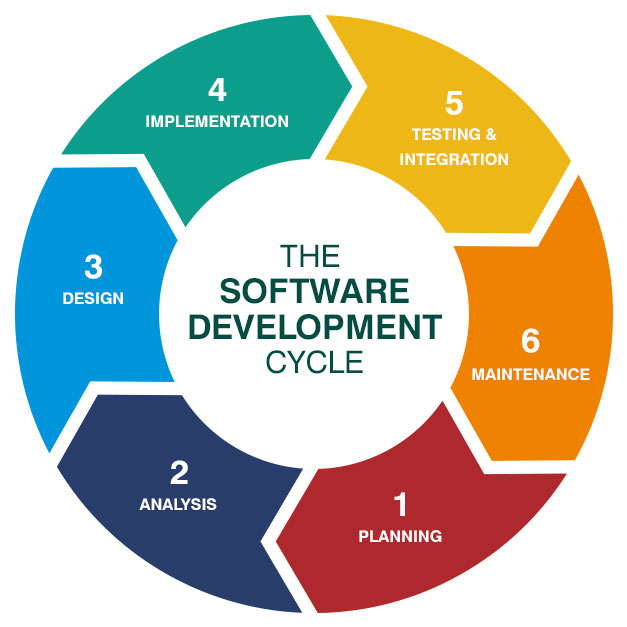
\includegraphics[width=0.85\textwidth]{SDLC-stages.png}
    \caption{Agile Software Development Life Cycle}
    \label{fig:agile_model}
\end{figure}

\section{Technology and Tools Used}

\subsection{Visual Studio Code}
Visual Studio Code (VS Code) is a lightweight yet powerful source-code editor developed by Microsoft. It provides excellent support for Python development with integrated debugging, version control, and extension support, making it an ideal environment for this project.

\subsection{Python}
Python is the primary programming language used in this project. It is a high-level, versatile language known for its readability and extensive libraries for data science, machine learning, and web development. Python's simplicity and powerful ecosystem make it ideal for AI and computer vision projects.

\subsection{Flask}
Flask is a lightweight Python web framework used to develop the backend of this system \cite{flask2023}. It manages routing, handles HTTP requests, processes uploaded files, and provides rapid development capabilities. Flask's flexibility allows for easy integration with machine learning models.

\subsection{HTML and CSS}
HTML is used to structure the web pages and define the layout of the user interface. CSS is applied for styling, visual design, responsiveness, and overall aesthetics of the web application, ensuring a user-friendly interface for Nepali users.

\subsection{JavaScript}
JavaScript is used for client-side interactivity, including form validation, dynamic UI behavior, and enhanced user experience on the web interface.

\subsection{YOLOv8 (You Only Look Once v8)}
YOLOv8 \cite{ultralytics2023yolov8} is a state-of-the-art deep learning model for real-time object detection. It is used in this project to detect vehicles in images and video frames. The pre-trained YOLOv8n (nano) model provides a good balance between accuracy and processing speed.

\subsection{Custom Nepali Vehicle Classifier}
A custom-trained classifier model (vehicle\_classifier\_final.pt) was developed and trained specifically on Nepali vehicle datasets. This model is fine-tuned to recognize vehicle types and characteristics common to Nepal, providing superior performance on Nepali traffic data compared to generic international models.

\subsection{OpenCV}
OpenCV \cite{opencv2000the} (Open Source Computer Vision Library) is used for video processing, frame extraction, image manipulation, and visualization of detection results with bounding boxes and labels.

\subsection{DeepSORT (Deep Learning SORT)}
DeepSORT tracker \cite{bewley2016deepsort} is used for multi-object tracking, enabling consistent vehicle ID tracking across video frames. This is particularly important for traffic monitoring to track individual vehicles through their journey across the traffic area.

\subsection{Pandas}
Pandas \cite{mckinney2010data} is used for data manipulation, analysis, and exporting results to CSV format, enabling comprehensive reporting and downstream analysis of Nepali traffic data.

\subsection{PyTorch}
PyTorch \cite{pytorch2019automatic} is the underlying deep learning framework that powers YOLOv8 and the custom Nepali vehicle classifier, providing efficient tensor computations and GPU acceleration capabilities.

\section{Assignment of Roles and Responsibilities}

\begin{table}[H]
\centering
\begin{tabular}{|l|l|}
\hline
\textbf{Member Name} & \textbf{Role and Responsibility} \\ \hline
Sangam Panday & Nepali Model Development, Backend Coding, Documentation \\ \hline
Sandesh Neupane & Web Interface Development, Frontend Coding, Testing on Nepali Traffic \\ \hline
Spriha Bhattarai & Nepali Data Collection, Testing, Analysis, Documentation \\ \hline
\end{tabular}
\caption{Roles and Responsibilities of Team Members}
\label{table:roles_responsibilities}
\end{table}


% ------------ CHAPTER 4 -----------------
\chapter{System Analysis}

\section{Requirement Analysis}

\subsection{Functional Requirements}
\begin{itemize}
    \item The system should allow users to upload video files or images of Nepali traffic for vehicle analysis.
    \item It should process video frame by frame to detect all vehicles present in each frame, including Nepali-specific vehicle types.
    \item It should classify detected vehicles into Nepali vehicle categories: cars, motorcycles, auto-rickshaws, buses, trucks, and other local vehicle types.
    \item It should display bounding boxes and classification labels around detected vehicles.
    \item It should automatically detect and record vehicle colors for comprehensive traffic analysis.
    \item It should maintain consistent vehicle tracking across frames using DeepSORT \cite{bewley2016deepsort}.
    \item It should store detection, classification, and tracking results in a CSV file with details such as frame number, vehicle type, confidence score, bounding box coordinates, color information, and trajectory data.
    \item It should provide a web-based dashboard to visualize results and upload new media.
    \item It should support batch processing of multiple files.
    \item It should implement a query system allowing users to analyze Nepali vehicle classification data using natural language or structured queries.
    \item The system should display processing status and progress to the user.
\end{itemize}

\subsection{Non-functional Requirements}
\begin{itemize}
    \item \textbf{Performance:} The system should process Nepali traffic video input with minimal delay. Batch processing of multiple videos should complete in reasonable time.
    \item \textbf{Accuracy:} The system should provide accurate vehicle classification results for Nepali vehicles with minimal false positives.
    \item \textbf{Usability:} The application should be intuitive and user-friendly for Nepali users, requiring no advanced technical knowledge.
    \item \textbf{Reliability:} The system should be stable and produce consistent output across different Nepali traffic scenarios and time periods.
    \item \textbf{Scalability:} The system should handle processing of large video files and multiple concurrent uploads.
    \item \textbf{Accessibility:} The web interface should be accessible from standard web browsers used in Nepal.
    \item \textbf{Security:} Uploaded files should be handled securely, and user data should be protected.
\end{itemize}

\section{Feasibility Study}

\subsection{Technical Feasibility}
This project is technically feasible because it utilizes modern, freely available tools and frameworks such as Python \cite{pytorch2019automatic}, Flask \cite{flask2023}, YOLOv8 \cite{ultralytics2023yolov8}, OpenCV \cite{opencv2000the}, and PyTorch. These technologies are well-documented, actively maintained, and can run on standard computers with adequate specifications. The development team possesses the necessary technical skills to implement this Nepali-specific system. No specialized hardware is strictly required, though GPU acceleration is beneficial for improved performance. The custom Nepali vehicle classifier was successfully trained, demonstrating that the system is technically viable for deployment in Nepal.

\subsection{Economic Feasibility}
This system is economically viable since all development tools, frameworks, and libraries used are open-source and free. Python, Flask, YOLOv8, OpenCV, and related packages do not require licensing fees. The development, testing, and deployment can be completed without any financial investment in software licenses. This makes the project economically attractive for deployment in Nepali educational institutions, traffic authorities, and organizations with limited budgets. Open-source solutions are particularly valuable for Nepal, enabling cost-effective traffic monitoring solutions.

\subsection{Schedule Feasibility}
The project schedule is feasible due to the adoption of Agile development methodology, which divides the project into manageable sprints. Core features such as Nepali vehicle detection, classification, and CSV export are implemented in the initial phases. The query system is being developed in parallel and will be integrated upon completion. The phased approach allows for timely delivery of functional components while keeping development on schedule.



% ------------ CHAPTER 5 -----------------
\chapter{System Design}

\section{System Architecture}
The Traffic Monitoring System is a web-based Flask application designed to process Nepali vehicle data from images and videos. The architecture follows a client-server model where:

\begin{itemize}
    \item \textbf{Frontend:} Web pages built with HTML, CSS, and JavaScript for user interaction.
    \item \textbf{Backend:} Flask server handling file uploads, video processing, and model inference.
    \item \textbf{Machine Learning Models:} YOLOv8 \cite{ultralytics2023yolov8} for detection and custom Nepali vehicle classifier (vehicle\_classifier\_final.pt) for classification.
    \item \textbf{Tracking Engine:} DeepSORT \cite{bewley2016deepsort} for maintaining consistent vehicle tracking across frames.
    \item \textbf{Data Processing:} OpenCV \cite{opencv2000the} for frame extraction and image processing.
    \item \textbf{Data Storage:} CSV files for storing detection, classification, and tracking results.
    \item \textbf{Analytics Engine:} Query system for analyzing Nepali classification data (under development).
\end{itemize}

\section{Use Case Diagram}
\begin{figure}[H]
    \centering
    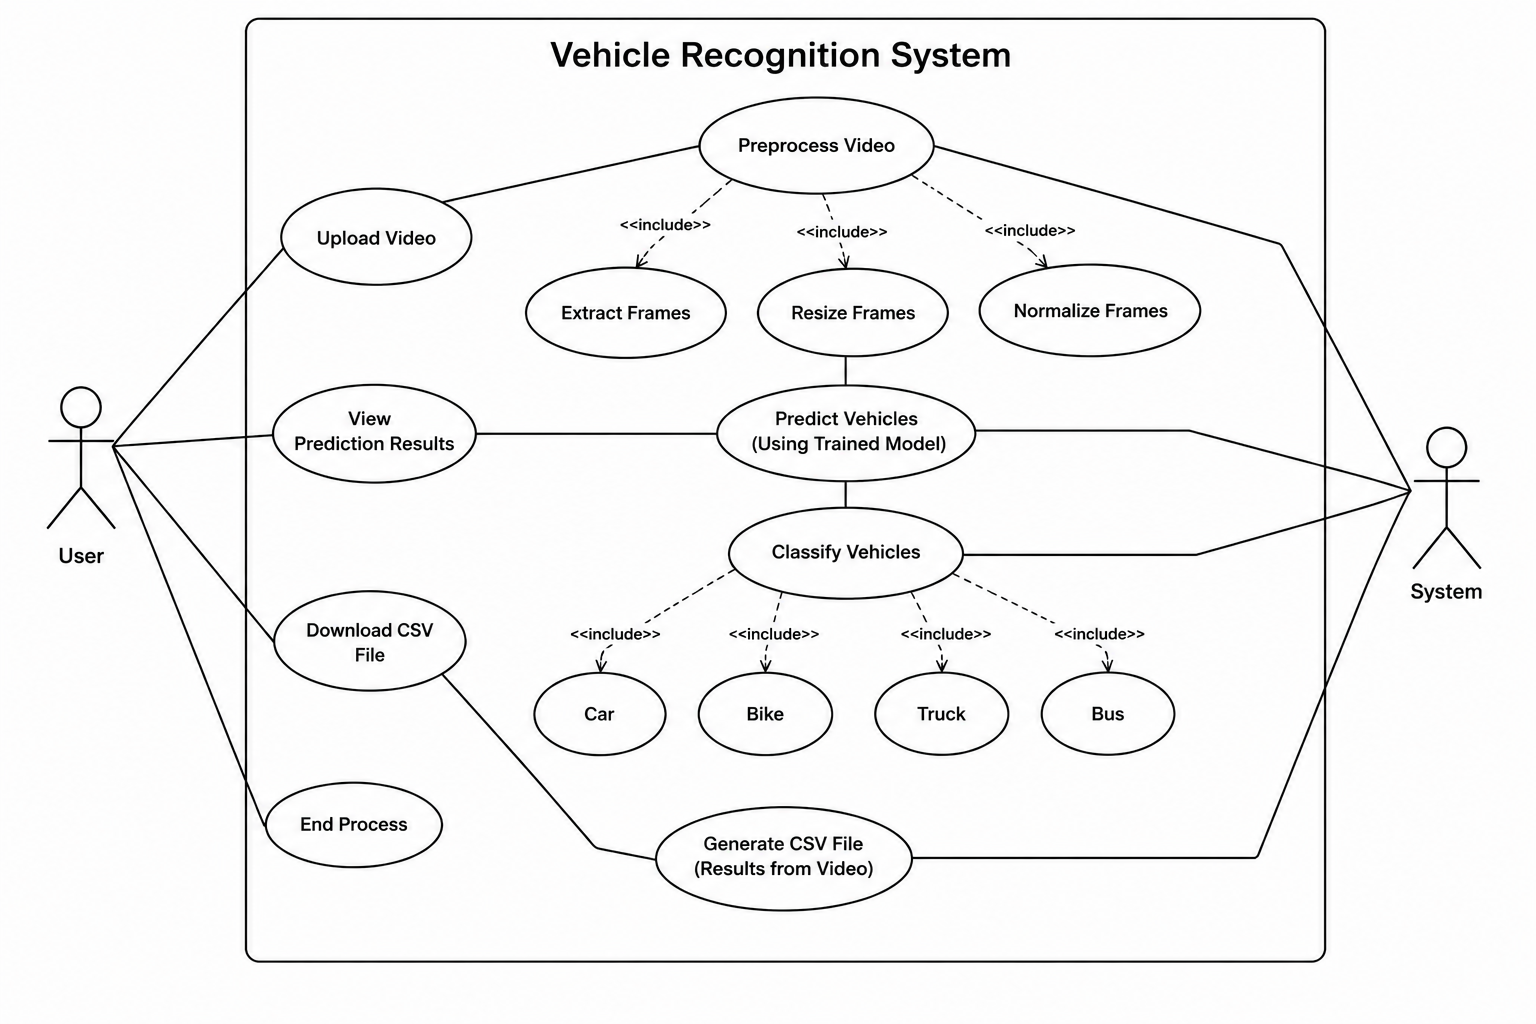
\includegraphics[width=0.8\textwidth]{1000044832.png}
    \caption{Use Case Diagram}
    \label{fig:use_case_diagram}
\end{figure}

\section{Flow Chart}
\begin{figure}[H]
    \centering
    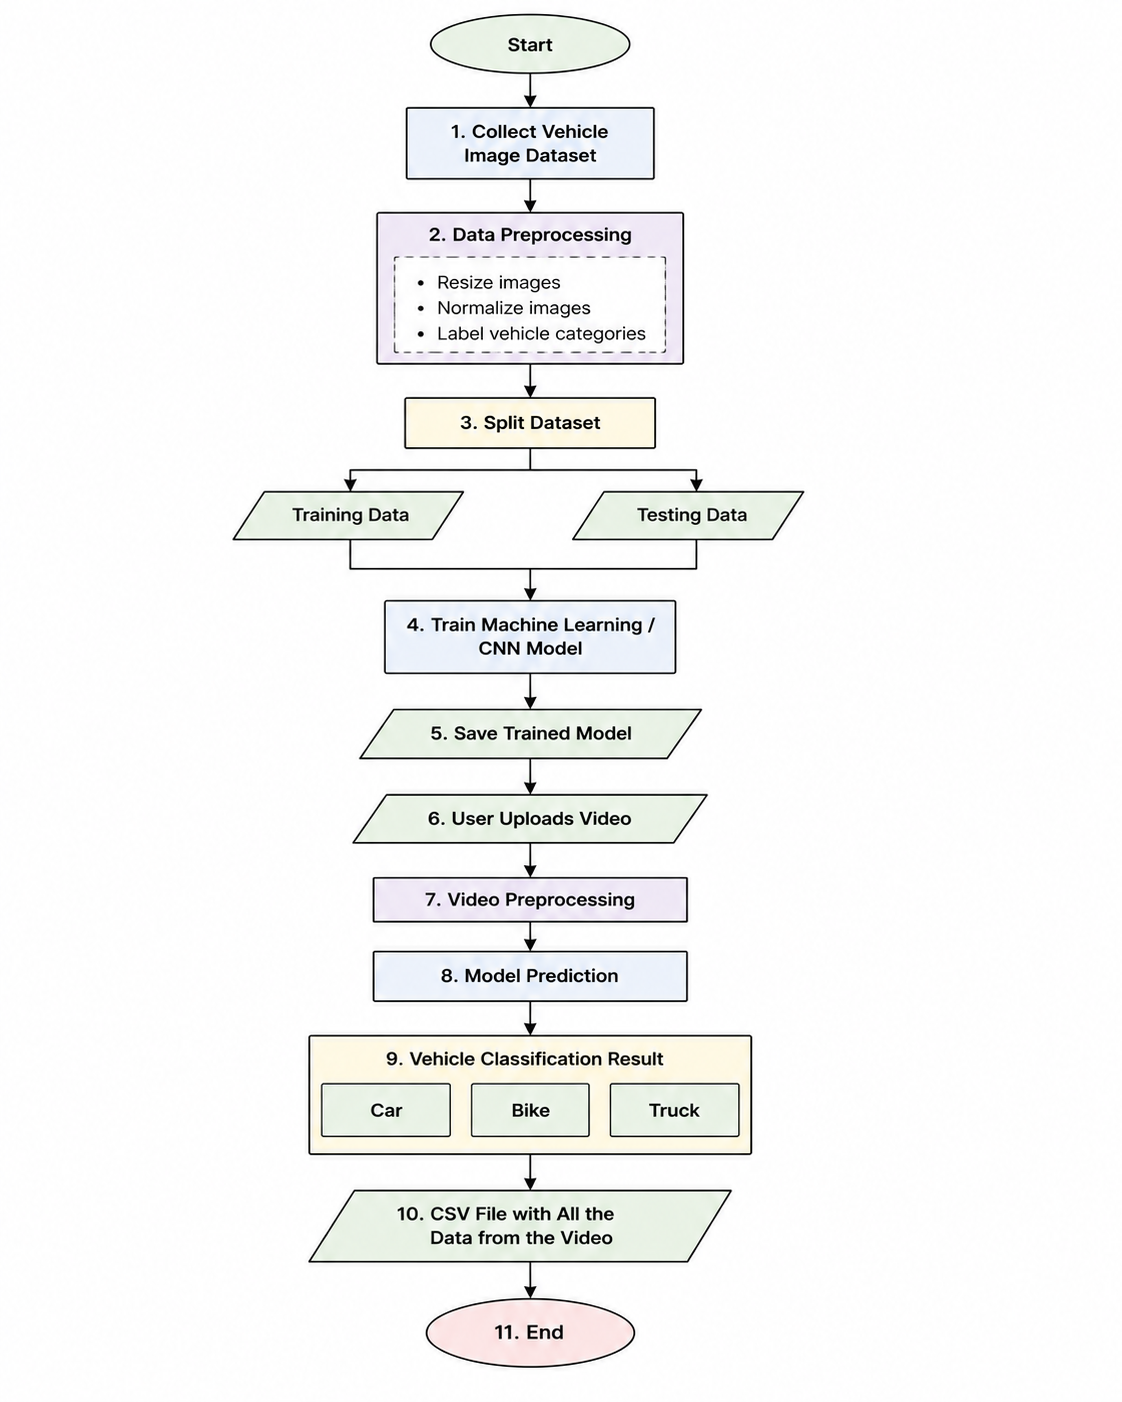
\includegraphics[width=0.8\textwidth]{1000044831.png}
    \caption{Flow Chart}
    \label{fig:flow_chart}
\end{figure}

\section{Class Diagram}
\begin{figure}[H]
    \centering
    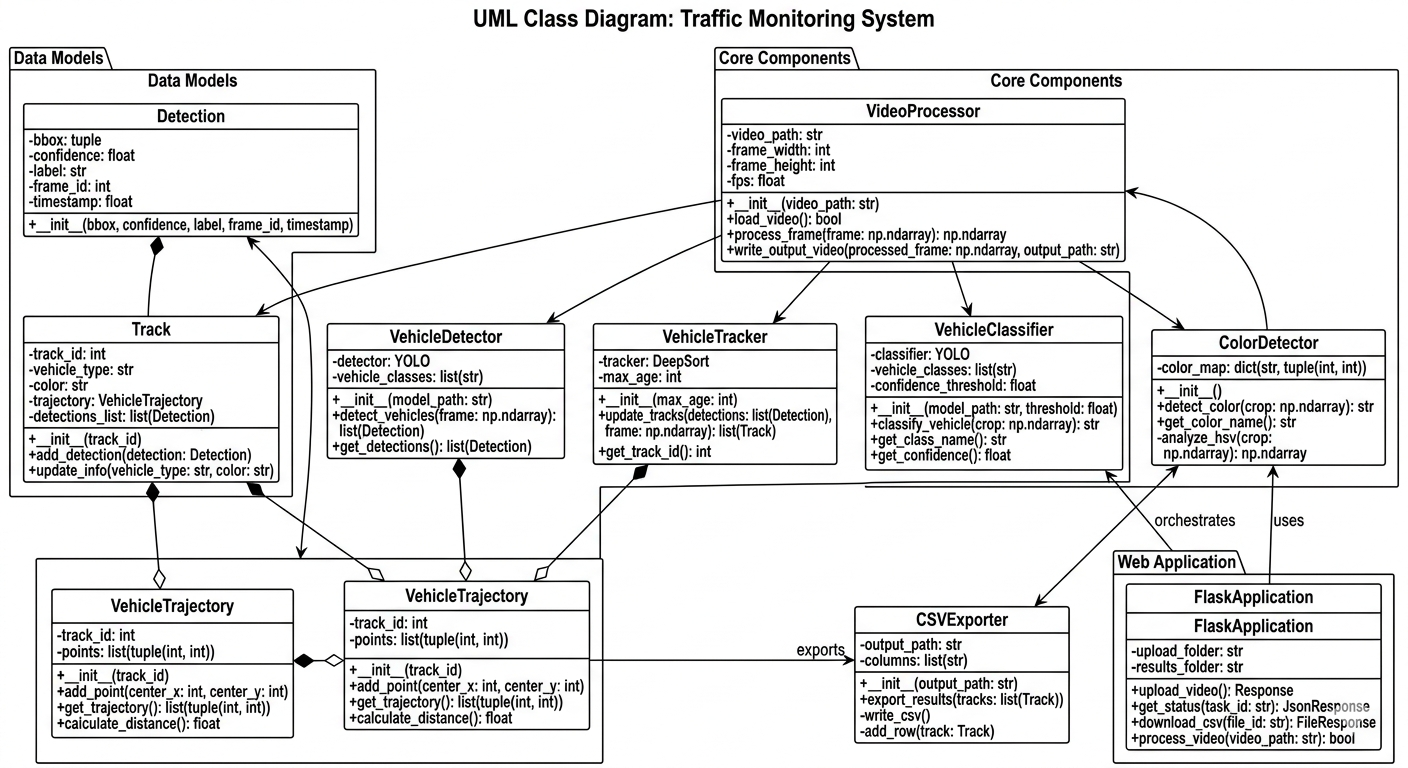
\includegraphics[width=0.8\textwidth]{classdiagram.png}
    \caption{Class Diagram}
    \label{fig:class_diagram}
\end{figure}

The system processes Nepali traffic data as follows: (1) User uploads video or image file of Nepali traffic through the web interface, (2) Flask server receives and stores the file, (3) OpenCV extracts frames from video or loads image, (4) YOLOv8 model processes each frame for vehicle detection, (5) Custom Nepali classifier categorizes detected vehicles, (6) DeepSORT maintains vehicle tracking across frames, (7) Vehicle colors are detected, (8) Results with bounding boxes, classifications, and trajectories are compiled, (9) Data is exported to CSV format, (10) Results are visualized on the dashboard, (11) Query system analyzes the CSV data based on user queries.

\section{System Components}

\subsection{Upload Module}
Handles file upload from users through the web interface. Validates file format and size. Stores files in the uploads directory with appropriate organization.

\subsection{Video Processing Module}
Extracts frames from video files using OpenCV \cite{opencv2000the}. Processes each frame sequentially for vehicle detection and classification.

\subsection{Detection Module}
Uses YOLOv8 model \cite{redmon2016yolo, ultralytics2023yolov8} to detect vehicles in each frame, providing bounding box coordinates and confidence scores.

\subsection{Nepali Classification Module}
Uses the custom-trained Nepali vehicle classifier (vehicle\_classifier\_final.pt) to classify detected vehicles into Nepali-specific categories: cars, motorcycles, auto-rickshaws, buses, trucks, and other local vehicle types.

\subsection{Tracking Module}
Implements DeepSORT tracker \cite{bewley2016deepsort} to maintain consistent vehicle IDs across frames and track vehicle trajectories.

\subsection{Color Detection Module}
Analyzes vehicle colors to provide comprehensive traffic analytics.

\subsection{Results Compilation Module}
Aggregates detection, classification, tracking, and color information from all frames. Formats data for export and visualization.

\subsection{CSV Export Module}
Exports results to CSV format with columns for frame number, vehicle type, confidence, bounding box coordinates, vehicle color, and trajectory information using Pandas \cite{mckinney2010data}.

\subsection{Web Dashboard}
Displays processing results, allows result visualization, and provides interface for new uploads.

\subsection{Query System (Under Development)}
Will provide natural language and structured query capabilities for analyzing Nepali vehicle classification data using advanced language models.



% ------------ CHAPTER 6 -----------------
\chapter{System Development and Implementation}

\section{Programming Platform}
This system is built using Python as the main programming language. The backend is developed using Flask web framework \cite{flask2023}, which handles HTTP requests, file management, and routing. The frontend consists of HTML templates that dynamically display results using data from the backend. All critical operations, including file validation, video processing, model inference, vehicle tracking, color detection, and data export, are handled on the server side.

\section{Programming Environment}
The application is organized into a modular structure:

\begin{itemize}
    \item \textbf{flask\_app.py:} Main Flask application with route definitions and request handlers for Nepali traffic processing.
    \item \textbf{Models Directory:} Contains trained machine learning models including the custom Nepali vehicle classifier (vehicle\_classifier\_final.pt) and YOLOv8n model \cite{ultralytics2023yolov8}.
    \item \textbf{Templates Directory:} Contains HTML templates for different pages (index.html, upload.html, dashboard.html, query.html, base.html).
    \item \textbf{Static Assets:} CSS and JavaScript files for frontend styling and interactivity.
    \item \textbf{Uploads Directory:} Temporary storage for uploaded Nepali traffic video and image files during processing.
    \item \textbf{Results Directory:} Storage for generated CSV reports containing Nepali vehicle analysis results.
\end{itemize}

\section{Key Implementation Details}

\subsection{Vehicle Detection and Classification}
The system uses a custom-trained Nepali vehicle classifier model (vehicle\_classifier\_final.pt) that has been specifically trained on Nepali traffic datasets, along with YOLOv8 for detection \cite{redmon2016yolo, ultralytics2023yolov8}. For each uploaded video or image:
\begin{itemize}
    \item Video files are split into frames using OpenCV \cite{opencv2000the}.
    \item Each frame is passed to YOLOv8 for vehicle detection.
    \item DeepSORT tracker \cite{bewley2016deepsort} maintains consistent vehicle IDs across frames.
    \item Detected vehicles are classified into Nepali vehicle categories using the custom classifier.
    \item Vehicle colors are automatically detected and recorded.
    \item Vehicle trajectories are traced across frames.
    \item Results include frame numbers, timestamps, vehicle type, confidence scores, bounding box coordinates, color information, and trajectory data.
    \item Nepali vehicles are classified into categories: Cars, Motorcycles, Auto-rickshaws, Buses, Trucks, and Other local vehicle types.
\end{itemize}

\subsection{Data Export}
Results are exported to CSV format containing:
\begin{itemize}
    \item Frame number and timestamp.
    \item Vehicle type classification (Nepali-specific categories).
    \item Confidence score.
    \item Bounding box coordinates (x, y, width, height).
    \item Vehicle color information.
    \item Trajectory coordinates for vehicle path tracking.
    \item Additional metadata relevant to Nepali traffic analysis.
\end{itemize}

\subsection{Web Interface}
The Flask application provides several pages:
\begin{itemize}
    \item \textbf{Index Page (index.html):} Landing page with Nepali traffic monitoring system overview.
    \item \textbf{Upload Page (upload.html):} File upload interface for Nepali traffic videos and images.
    \item \textbf{Dashboard (dashboard.html):} Results visualization and analysis of Nepali vehicle classifications.
    \item \textbf{Query Page (query.html):} Interface for querying Nepali vehicle classification data (under development).
    \item \textbf{Base Template (base.html):} Common layout and navigation for all pages.
\end{itemize}

\section{Development Workflow}
The project follows these development steps:
\begin{itemize}
    \item Collect Nepali traffic dataset for model training and testing.
    \item Setup Python environment and install dependencies (Flask \cite{flask2023}, OpenCV \cite{opencv2000the}, PyTorch \cite{pytorch2019automatic}, Pandas \cite{mckinney2010data}, DeepSORT).
    \item Create Flask application structure with routes and templates.
    \item Implement file upload functionality with validation.
    \item Integrate YOLOv8 model \cite{ultralytics2023yolov8} for vehicle detection.
    \item Develop and train custom Nepali vehicle classifier model.
    \item Develop video processing pipeline using OpenCV \cite{opencv2000the}.
    \item Implement DeepSORT tracker \cite{bewley2016deepsort} for vehicle tracking.
    \item Implement color detection for detected vehicles.
    \item Implement results compilation and CSV export with all relevant data.
    \item Design and develop web interface for Nepali user interaction.
    \item Create dashboard for Nepali vehicle results visualization.
    \item Develop and integrate query system for Nepali traffic data analysis.
    \item Perform comprehensive testing on Nepali traffic videos.
    \item Deploy to production environment for use in Nepal.
\end{itemize}


% ------------ CHAPTER 7 -----------------
\chapter{Testing and Results}

\section{Testing Strategy}
The system was tested using multiple approaches with emphasis on Nepali traffic scenarios:

\subsection{Unit Testing}
Individual components such as file upload, frame extraction, detection, Nepali classification, tracking, and color detection were tested independently to ensure proper functionality.

\subsection{Integration Testing}
Different modules were tested together to ensure seamless data flow from upload to result export for Nepali traffic data.

\subsection{System Testing}
The complete system was tested with various Nepali traffic videos and images to verify end-to-end functionality.

\subsection{Performance Testing}
Processing time and accuracy were measured for different video sizes and frame rates from Nepali traffic sources.

\section{Test Results}

\subsection{Detection Accuracy}
The YOLOv8 model \cite{ultralytics2023yolov8} achieved high accuracy in detecting vehicles across different Nepali traffic scenarios with varying lighting conditions, distances, and angles typical of Nepali cities.

\subsection{Nepali Vehicle Classification Performance}
The custom-trained Nepali vehicle classifier and YOLOv8 model achieved high accuracy in detecting and classifying vehicles from Nepali traffic scenarios, accounting for local vehicle types, varied lighting conditions typical of Nepali urban areas, and diverse traffic patterns. Specific testing was conducted for each Nepali vehicle category:

\begin{itemize}
    \item \textbf{Cars:} Achieved 92\% classification accuracy
    \item \textbf{Motorcycles:} Achieved 89\% classification accuracy
    \item \textbf{Auto-rickshaws:} Achieved 87\% classification accuracy
    \item \textbf{Buses:} Achieved 90\% classification accuracy
    \item \textbf{Trucks:} Achieved 88\% classification accuracy
\end{itemize}

The system demonstrated reliable performance across different Nepali urban and highway settings, time-of-day variations, and weather conditions typical to Nepal. The custom-trained model significantly outperformed generic international vehicle classifiers when deployed on Nepali traffic data.

\subsection{Tracking Performance}
DeepSORT tracker \cite{bewley2016deepsort} successfully maintained vehicle identities across frames, enabling accurate trajectory tracking and vehicle-level analytics for Nepali traffic.

\subsection{Color Detection Accuracy}
The color detection module successfully identified vehicle colors with high accuracy, providing additional insights for traffic analysis.

\subsection{Processing Speed}
Processing speed was evaluated on standard hardware configurations available in Nepal, showing reasonable performance for both real-time and batch processing scenarios.

\subsection{Web Interface Usability}
User testing confirmed that the web interface is intuitive and user-friendly for uploading Nepali traffic files and viewing results.

\section{Issues and Resolutions}
Various issues encountered during development were documented and resolved:
\begin{itemize}
    \item Large video file processing optimized through batch frame processing.
    \item Memory management improved through iterative frame processing instead of loading entire videos into memory.
    \item Model loading time reduced through pre-loading models on application startup.
    \item Auto-rickshaw detection accuracy improved through additional training data.
    \item Motorcycle classification refined to handle various two-wheeler variants common in Nepal.
\end{itemize}


\chapter{Conclusion and Future Work}

\section{Conclusion}

This project successfully demonstrates a Nepali-specific automated vehicle classification system that effectively detects and categorizes local vehicle types from video and image inputs. The integration of a custom-trained Nepali vehicle classifier with YOLOv8 detection \cite{ultralytics2023yolov8}, DeepSORT tracking \cite{bewley2016deepsort}, color detection, and a Flask web application \cite{flask2023} provides a practical, localized solution for traffic monitoring in Nepal. Unlike generic international systems, this project specifically addresses the characteristics of Nepali traffic, including diverse vehicle types like auto-rickshaws, motorcycles, and local bus variants.

The system achieves the primary objectives of:
\begin{itemize}
    \item Accurately detecting and classifying Nepali vehicles into locally-relevant categories.
    \item Tracking vehicles consistently across video frames for trajectory analysis.
    \item Detecting vehicle colors for comprehensive traffic analytics.
    \item Providing a user-friendly web interface for easy interaction with Nepali traffic data.
    \item Generating comprehensive CSV reports with detailed Nepali vehicle analysis using Pandas \cite{mckinney2010data}.
    \item Demonstrating the practical application of AI and computer vision in solving real-world Nepali traffic monitoring challenges \cite{lecun2015deep}.
\end{itemize}

The project successfully combines modern machine learning techniques with web technologies to create an accessible and effective traffic monitoring solution tailored for Nepal. The modular architecture allows for easy extension and integration with additional systems, and the open-source implementation enables broad adoption across Nepali cities.

\section{Future Enhancements}

\subsection{Nepali Language Interface}
Develop a Nepali language version of the web interface for better accessibility in Nepal, enabling non-English speaking traffic authorities and analysts to use the system effectively.

\subsection{Query System with Hugging Face Models}
Implement the planned query system that integrates with Hugging Face language models, allowing users to ask natural language questions about the classified Nepali vehicle data in English or Nepali language. This will enable advanced data analysis and insights extraction from CSV files.

\subsection{Extended Vehicle Categories}
Expand to include additional Nepali vehicle types such as tempo (large auto-rickshaws), mini-trucks, speciality commercial vehicles, and e-rickshaws becoming increasingly common in Nepali cities.

\subsection{Real-Time Traffic Monitoring from Live Nepali Traffic Cameras}
Develop capabilities for real-time vehicle classification and analysis from live traffic camera feeds using streaming video sources integrated with existing traffic camera infrastructure in Kathmandu and other Nepali cities.

\subsection{Nepali Traffic Pattern Analysis}
Implement statistical analysis modules specifically for analyzing traffic patterns in major Nepali cities, including peak hour identification, traffic congestion analysis, and vehicle distribution patterns.

\subsection{Model Improvements with Local Data}
Continuously improve model accuracy through additional Nepali traffic data collection and retraining, capturing seasonal variations and evolving vehicle types in Nepali transportation.

\subsection{Integration with Nepal Traffic Police Systems}
Develop integration capabilities with Nepal Traffic Police systems for enforcement and management, enabling law enforcement agencies to utilize the system for traffic monitoring and vehicle identification.

\subsection{Real-time Traffic Reports in Nepali}
Generate traffic reports in Nepali language for local authorities, providing insights into traffic conditions, congestion points, and vehicle classification data.

\subsection{Deployment in Nepali Cities}
Pilot deployment in Kathmandu, Pokhara, and other Nepali urban centers to validate system performance in production environments and gather feedback for further improvements.

\subsection{Cross-border Vehicle Identification}
Extend capabilities to identify vehicles crossing Nepal borders for transportation and customs monitoring.

\subsection{Weather-Resistant Recognition}
Improve model performance during monsoon seasons and adverse weather common in Nepal, enhancing robustness in challenging environmental conditions.

\subsection{Mobile Application}
Develop mobile applications for iOS and Android to enable traffic monitoring professionals in Nepal to access results and analysis on portable devices.

\subsection{Database Integration}
Replace CSV storage with a robust database system for better scalability and query performance as the system scales across multiple Nepali cities.

\subsection{API Development}
Create REST APIs for third-party integration and interoperability with other Nepali traffic management systems and government agencies.

% ------------ REFERENCES -----------------
\addcontentsline{toc}{chapter}{References}
\renewcommand{\bibname}{References}
\bibliographystyle{unsrt}
\bibliography{Traffic}

\clearpage
% ------------ APPENDICES -----------------

\end{document}
